%!TEX root = ./seminar.tex
\section{The Current State of Digital Health(care)}
\subsection{Costs}
Looking at the current state of healthcare in general around the world, we see a trend of increasing costs year by year. Estimations consider a global annual cost of \$8.7 trillion by 2020 in contrast to \$7 trillion in 2015. This corresponds to a steady 10\% of the GDP worldwide on average as can be seen in Figure~\ref{fig:GDPSpendingHC}.
\begin{figure}[htpb]
    \centering
    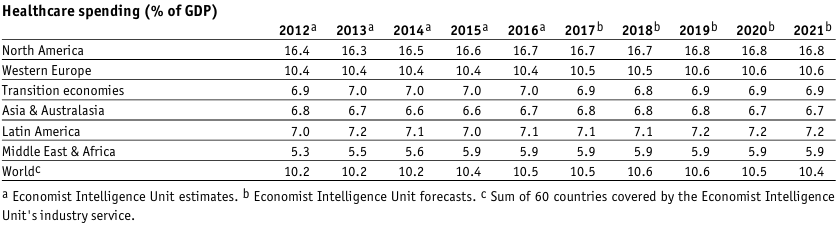
\includegraphics[width=\linewidth]{media/Screenshot_2020-01-09_01_FULL_REPORT-World_healthcare_and.png}
    \caption{Healthcare spending around the world \cite{EIU2016}}%
    \label{fig:GDPSpendingHC}
\end{figure}
Especially in North America and Europe this is due to increasing rates of multiple chronic conditions and age related diseases \cite{sambamoorthi2015multiple}. Another major contributor to rising healthcare cost are "preventable adverse drug events associated with inpatient injectable medications" \cite{lahue2012national}; With an estimated 7 million patients suffering the consequences in the United States they contribute to 7000 deaths and almost \$21 billion in direct medical costs across all care settings annually \cite{prevMedErrors}.
\subsection{Efficiency}
About 30\% of global data volume is generated by the healthcare industry \cite{gopal2019digital}, but healthcare data is among the slowest to be digitized \cite{industryDigitalization}. This leaves us with large quantities of data in unstructured and analog formats. The process to digitize them is prone to errors as well as time intense. Time, our healthcare systems do not have, as more and more patients with chronic diseases require said time \cite{ostbye2005there}. This results in less time healthcare professionals can spend with their patients \cite{fuchtbauer2013emergency} and therefore a decline in patient satisfactory \cite{gross1998patient}. With more frequent interactions due to chronic disease this inhibits a good relationship between doctors and their patients.
\subsection{Risks}
Healthcare environments should not allow even the smallest margin of error when it comes to the health outcome of patients. Still, illegible handwriting is far to common among physicians such that about a sixth of doctor's notes are unclear to others \cite{rodriguez2002illegible}. With the already seen costs of medication errors this is a huge risk factor for the healthcare environment. Further risks include misdiagnosis, accounting to 225,000 deaths each year in the United States alone \cite{gregerIatrogenic} and postoperative infections, occurring after approximately 2-5\% of surgeries and accounting for 17\% of hospital acquired infections \cite{andreu2015wearable}.

